%!TEX root = ../thesis.tex
%*******************************************************************************
%****************************** Third Chapter **********************************
%*******************************************************************************
\chapter{Diffusion models encode the intrinsic dimension of data manifolds}\label{Chapter:intrinsic-dimension}

% **************************** Define Graphics Path **************************
\ifpdf
    \graphicspath{{Chapter3/Figs/Raster/}{Chapter3/Figs/PDF/}{Chapter3/Figs/}}
\else
    \graphicspath{{Chapter3/Figs/Vector/}{Chapter3/Figs/}}
\fi

In this work, we provide a mathematical proof that diffusion models encode data manifolds by approximating their normal bundles. Based on this observation we propose a novel method for extracting the intrinsic dimension of the data manifold from a trained diffusion model. Our insights are based  on the fact that a diffusion model approximates the score function i.e. the gradient of the log density of a noise-corrupted version of the target distribution for varying levels of corruption. We prove that as the level of corruption decreases, the score function points towards the manifold, as this direction becomes the direction of maximal likelihood increase. Therefore, at low noise levels, the diffusion model provides us with an approximation of the manifold's normal bundle, allowing for an estimation of the manifold's intrinsic dimension.  To the best of our knowledge our method is the first estimator of intrinsic dimension based on diffusion models and it outperforms well established estimators in controlled experiments on both Euclidean and image data. The code is available at \url{https://github.com/GBATZOLIS/ID-diff}.

\section{Introduction}\label{ch3:sec:introduction}

Many modern real-world datasets contain a large number of variables, often exceeding the number of observations. This poses a major challenge in modelling them, due to the \textit{curse of dimensionality}. Despite this complexity,  due to the numerous relationships and symmetries among variables, even high-dimensional data often concentrates around a lower-dimensional manifold, a concept known as the \textit{manifold hypothesis} 
\cite{manifold_hypothesis}. The dimension of this manifold is called \textit{intrinsic dimension} (ID),  while the high-dimensional space in which the data resides is known as the
\textit{ambient space}, with its dimensionality called the \textit{ambient dimension}.

The manifold hypothesis has guided the development of modern high-dimensional data modelling techniques, such as Variational auto-encoders (VAEs) \cite{vae}, Generative Adversarial Networks (GANs) \cite{gan} and M-flows \cite{brehmer2020flows}. 

The estimation of ID holds significant importance in the machine learning community due to its applicability in both theoretical and practical problems \cite{campadelli2015intrinsic}. From a theoretical perspective, the ID is essential as it directly affects the convergence rates of fundamental statistical quantities \cite{weed2019sharp}. The higher the ID, the more data is needed for a model to generalize well beyond the training set \cite{campadelli2015intrinsic, pope2021intrinsic}, hence knowing the ID has numerous implications for the generalization and data efficiency of machine learning models \cite{kim2019kde, kpotufe2011knn}.  From practical point of view, ID is crucial for a wide range of dimensionality reduction methods \cite{campadelli2015intrinsic}.  Additionally, understanding the data's ID can help in fine-tuning the latent dimension of models such as GANs, VAEs or M-flows. 


In recent years, diffusion models \cite{diffusion_models, ddpm} emerged as a new class of deep generative models capable of capturing complex high-dimensional distributions without relying on the notion of data manifold or prior knowledge of the data's ID. Our research reveals that diffusion models encode data manifolds via their normal bundle. Intriguingly, we find that while diffusion models do not \textit{explicitly} rely on the ID, these models estimate it \textit{implicitly}.

As discussed in \cite{song2020score, ddpm}, diffusion models perform score matching \cite{score_matching} and, therefore, contain the information about the gradient of the log-density of the data distribution. We prove that near the data manifold, the gradient of the log-density is orthogonal to the manifold itself. This key observation serves as a tool for deducing the manifold's dimension.

In our study, we investigate three categories of ID estimators: traditional statistical methods (such as PCA and Nearest Neighbor based approaches), normalizing flow-based methods, and our innovative diffusion-based approach. We evaluate the performance of ID estimators  on synthetic Euclidean and image datasets, where the dimension of the data manifold is known \textit{a priori}. Moreover, we apply ID estimators to the MNIST dataset \cite{mnist} (where the ID is unknown), and compare the estimated IDs with the reconstruction error of auto-encoders trained with different latent dimensions. 

Our findings indicate that in datasets of high ID, methods that exploit the inductive biases of neural networks are the most effective. Our proposed method stands out by yielding the best results. This success is attributed to utilizing diffusion models, which offer enhanced training stability and avoid the architectural limitations associated with normalizing flows \cite{behrmann2021understandin}.

To summarize our contributions are as follows:
\begin{itemize}
    \item We elucidate a geometric connection between diffusion models and data manifolds, by proving that a diffusion model encodes the data manifold by approximating its normal bundle.
    \item Based on this observation we propose a novel method for extracting the ID of the data manifold from a trained diffusion model.
    \item We perform an extensive evaluation of our novel method as well as several prominent existing methods for ID estimation on a wide range of datasets.
\end{itemize}

\begin{figure}[h]
    \centering
    \begin{minipage}[t]{0.49\linewidth}
        \centering
        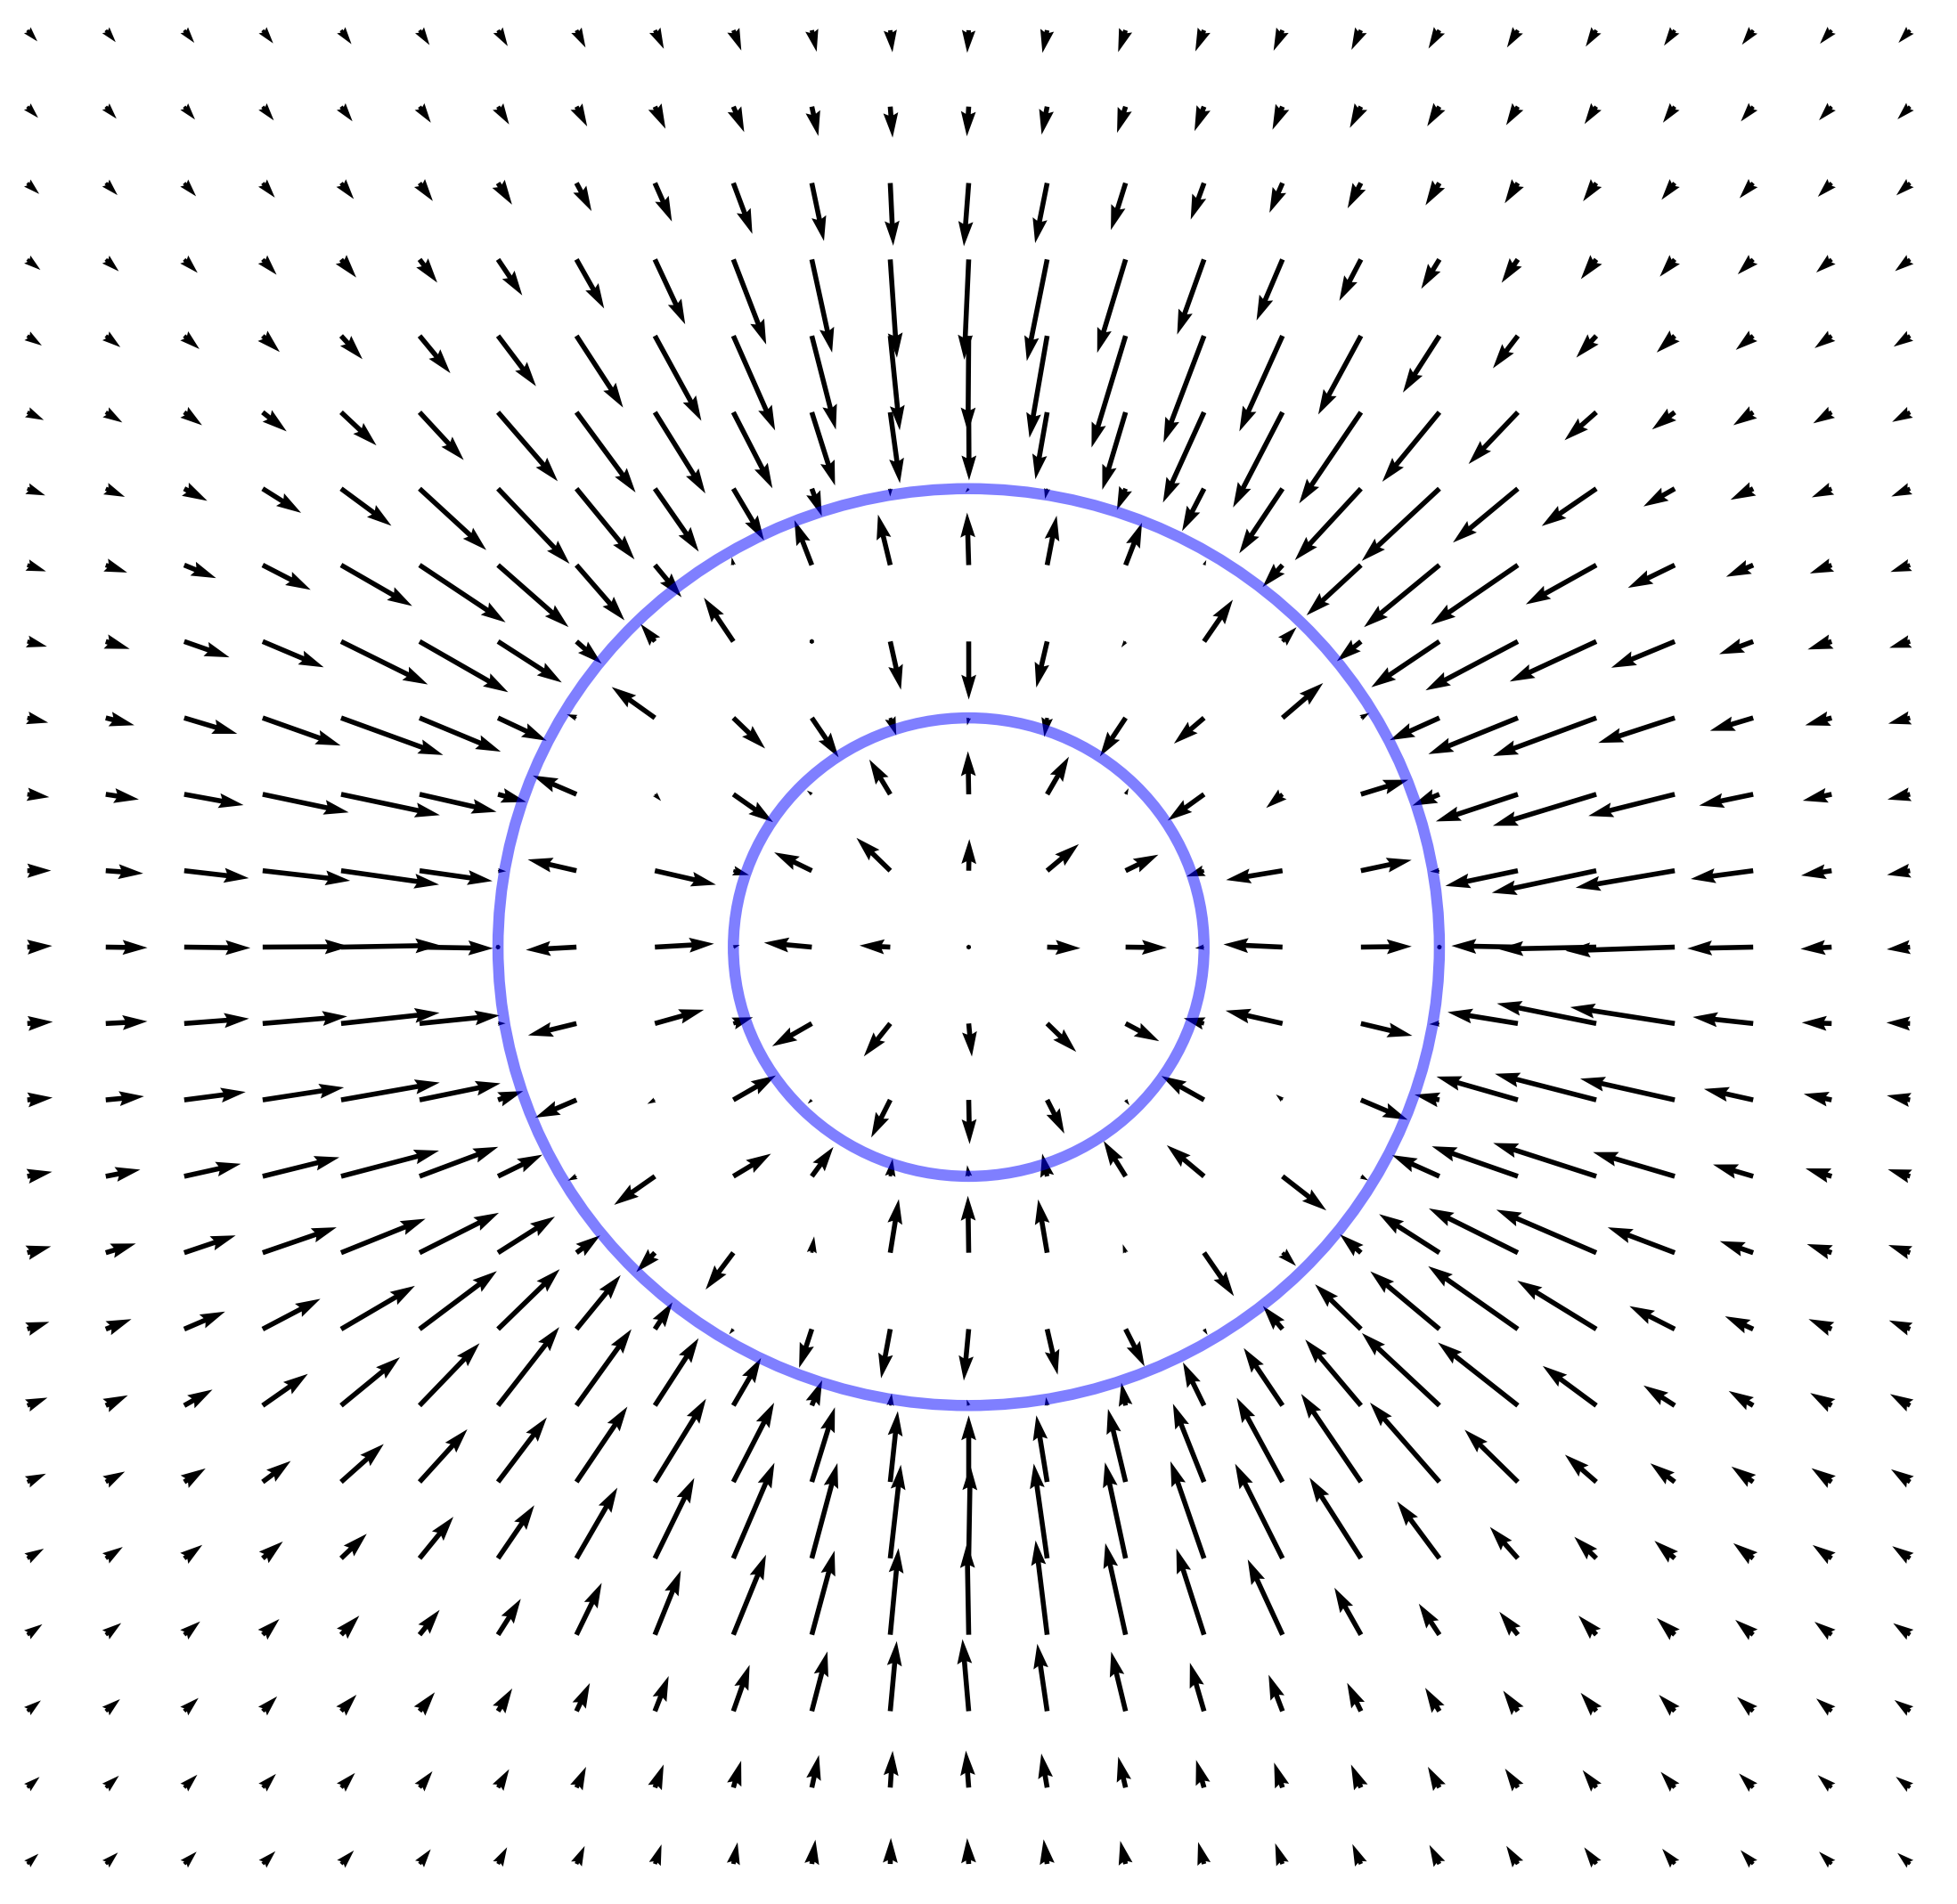
\includegraphics[width=\linewidth]{Chapter3/figures/score_field.png}
        \caption{The data manifold (in blue) and the neural approximation of the score field $\nabla_\textbf{x} \ln p_{t_0}(\textbf{x})$ obtained from a diffusion model. Near the manifold the score field is perpendicular to the manifold surface.}
        \label{ch3:fig:score_field}
    \end{minipage}
    \hfill
    \begin{minipage}[t]{0.49\linewidth}
        \centering
        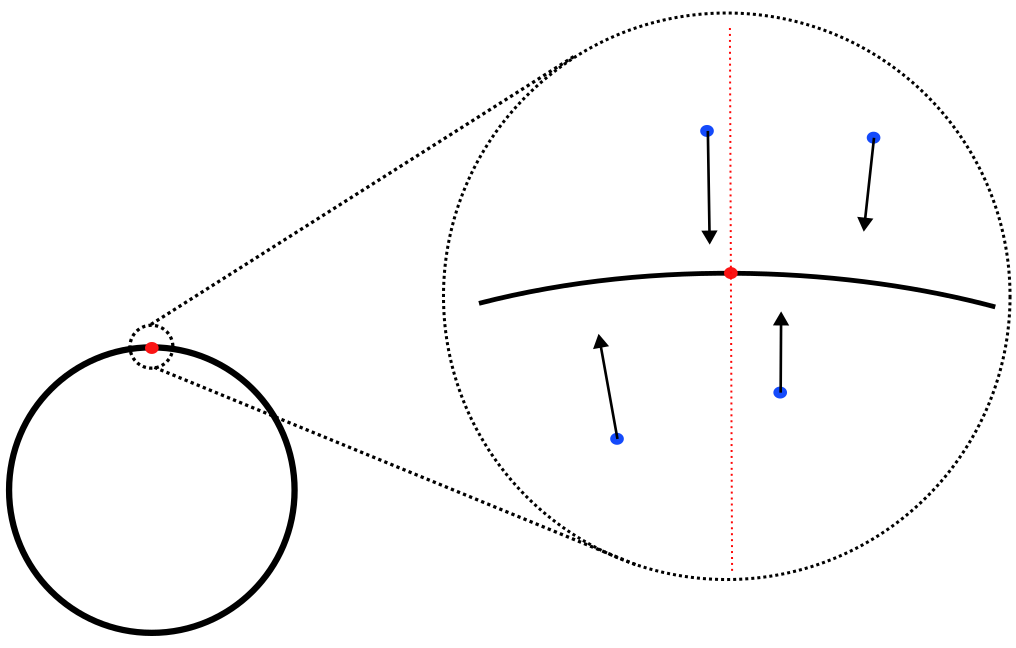
\includegraphics[width=\linewidth]{Chapter3/figures/drawing.png}
        \caption{To estimate the manifold's dimension at point \(\mathbf{x}_0\) (red dot), we sample \(K\) nearby points \(\mathbf{x}_{\epsilon}^{(i)}\) (blue dots) and use the trained diffusion model to evaluate the score function \(s_\theta(\mathbf{x}_\epsilon^{(i)}, \epsilon)\) at these perturbed points. We assemble these vectors into a matrix and perform Singular Value Decomposition (SVD). The number of (almost) zero singular values reveals the manifold's dimension.}
        \label{ch3:fig:zoom}
    \end{minipage}
\end{figure}


\section{Related Work}
\label{ch3:sec:related_work}
The relationship between diffusion models and manifold hypothesis has been explored in several recent works. In \cite{pidstrigach2022manifold_jakiw} author examines theoretical conditions under which diffusion models produce samples from the underlying data manifold. In \cite{oko2023diffusion_mini_max} and \cite{chen2023manifold_linear} authors analyze approximation and generalization abilities of diffusion models under manifold hypothesis. They establish that the data efficiency of training a diffusion model depends on the intrinsic dimension of the data manifold rather than the ambient dimension. This further motivates the importance of ID estimation.


The problem of estimating the intrinsic dimensionality has been widely studied. The two main lines of research are PCA based and nearest neighbour based approaches. In an early work \cite{Karhunen-Loeve} the authors suggest an approach based on using local Karhunen–Loève expansion. In following years many PCA based approaches have been developed. Most notably, in \cite{auto_ppca} the author suggests an intrinsic dimensionality estimator based on the probabilistic PCA (PPCA) framework \cite{ppca}. In \cite{fan_local_pca} a local PCA method has been suggested. In \cite{pettis_nn_dim_estimator} authors suggested an estimator based on nearest neighbour information.  In \cite{dim_MLE} authors introduce a maximum likelihood (MLE)  procedure based on the distance to $m$ nearest neighbours. Their method has been further improved in the work of \cite{haro_mle}. The MLE method has been recently applied by \cite{pope2021intrinsic} in the estimation of the intrinsic dimensionality of modern image datasets such as MNIST \cite{mnist}, CIFAR \cite{cifar} and ImageNet \cite{imagenet}. Other works explored geometric approaches using fractal-based methods \cite{fractal_dim} or packing numbers \cite{packing_number}. We refer to \cite{campadelli2015intrinsic} for a comprehensive survey of statistical approaches to ID estimation.

The aforementioned ID estimators do not leverage the inductive bias introduced by modern neural network architectures, which is a crucial reason for the success of modern deep leaning systems \cite{goyal2022inductive}. Therefore, their statistical efficiency may be insufficient to deal with datasets of high ID. This limitation has been observed in  \cite{campadelli2015intrinsic, horvat2022nfid} and is confirmed by our experimental findings.


The limitations of traditional statistical estimators have recently led to the development of deep learning-based intrinsic dimensionality (ID) estimators such as LIDL \cite{tempczyk2022lidl} and ID-NF \cite{horvat2022nfid}. These methods, which extract ID from trained normalizing flows, outperform their statistical counterparts by leveraging the inductive biases inherent in modern deep neural network architectures. Despite their advantages, they face challenges as they rely on normalizing flows which are invertible neural networks. Normalizing flows are subject to a trade-off between stability and expressivity, as discussed in \cite{behrmann2021understandin},\cite{jaini2020tails}, \cite{cornish2020relaxing},\cite{laszkiewicz2021copula}. Expressive normalizing flow architectures often face stability problems during training or evaluation, risking the reliability of post-training ID estimation due to potential loss of numerical invertibility. On the other hand, Lipschitz constrained normalizing flow architectures, while more stable, tend to be less expressive, potentially limiting their capacity to accurately estimate the ID of complex, high-dimensional data manifolds.

In contrast, our proposed methodology, which utilizes diffusion models, effectively sidesteps these expressivity limitations as diffusion models do not suffer from similar stability issues. Our method allows for more effective leveraging of the powerful inductive biases of modern deep neural network architectures, resulting in a more reliable and robust estimation of the ID of complex, high-dimensional data manifolds. This claim is further substantiated by our experimental findings, which show that our proposed diffusion-based estimation method accurates estimes the ID in challenging data manifolds where normalizing flow-based methods fail due to reduced expressivity.

\section{Proposed Method for Estimation of Intrinsic Dimension}
\label{ch3:sec:method}


\begin{algorithm}
    \caption{Estimate the Intrinsic Dimension at $\mathbf{x}_0$}
    \label{ch3:alg:intrinsic_dimension}
    \begin{algorithmic}[1]
        \STATE \textbf{Input:} $s_\theta$ - trained diffusion model, $\mathbf{x}_0$ - data point, $K$ - number of samples
        \STATE Sample $\mathbf{x}_0 \sim p_0(\mathbf{x})$ from the data set
        \STATE $d \gets \text{dim}(\mathbf{x}_0)$
        \STATE $S \gets$ empty matrix
        \FOR{$i = 1, \dots, K$}
            \STATE Sample $\mathbf{x}_{t_0}^{(i)} \sim \mathcal{N}(\mathbf{x}_0, \sigma^2 I)$
            \STATE Append $s_{\theta}(\mathbf{x}_{t_0}^{(i)}, t_0)$ as a new row in $S$
        \ENDFOR
        \STATE $(s_i)_{i=1}^d$, $(\mathbf{v}_i)_{i=1}^d$, $(\mathbf{w}_i)_{i=1}^d \gets \text{SVD}(S)$
        \STATE $\hat{k}(\mathbf{x}_0) \gets d - \argmax_{i=1,\dots,d-1} (s_i - s_{i+1})$
        \STATE \textbf{Output:} $\hat{k}(\mathbf{x}_0)$
    \end{algorithmic}
\end{algorithm}
    

In \cite{song2020score} score-based  \cite{score_matching} and diffusion-based \cite{diffusion_models, ddpm} generative models were unified into a single continuous-time score-based framework. The diffusion process is represented by a stochastic differential equation (SDE), which perturbs data distribution $p_0$  resulting in a series of progressively noise-corrupted distributions  $p_t$.  Diffusion models are trained to approximate the score function $\nabla_{\textbf{x}_t}{\ln{p_t(\textbf{x}_t)}}$ with a neural network $s_\theta(\textbf{x}_t,t)$. Once the score function is approximated, the diffusion SDE can be reversed to generate samples from $p_0$. Additional details on training and sampling from diffusion models are described in Appendix \ref{ch3:appendix:background}.
 
Consider a dataset $D=\{\textbf{x}^{(i)}\}_{i=0}^N\sim p_0(\textbf{x})$ which consists of $N$ independent $d$-dimensional vectors $\textbf{x}^{(i)} \in \mathbb{R}^d$ drawn from distribution $p_0(\textbf{x})$. The distribution $p_0(\textbf{x})$ is supported on a $k$-dimensional manifold $\mathcal{M}$, which is embedded in a space of ambient dimension $d$. Our goal is to infer the dimension $k$ of the manifold $\mathcal{M}$ from $D$.

We perturb the data according to the variance exploding SDE \(d\textbf{x}_t = g(t)d\textbf{w}_t\)  \cite{song2020score} and train a neural network $s_{\theta}(\textbf{x}_t,t)$ to approximate the score function of the noise perturbed target distribution, i.e. $\nabla_{\textbf{x}_t}{\ln{p_t(\textbf{x}_t)}}$ for a range of levels of perturbation indexed by diffusion time $t$. We train the model using the weighted denoising score matching objective with likelihood weighting, see \cite{song2021maximum}. More details about the training of the diffusion model can be found in Appendix \ref{ch3:sec:hparams}.

Consider a datapoint $\textbf{x}_0$ on a manifold $\mathcal{M}$ and its perturbation into the ambient space $\textbf{x}_{t_0}$ obtained from the transition kernel $p_{t_0}(\textbf{x}_{t_0} | \textbf{x}_0) = \mathcal{N}(\textbf{x}_{t_0} | \textbf{x}_0, \sigma^2_{t_0}\textbf{I})$\footnote{The transition kernels of the variance exploding SDE have this structure, where $\sigma_t$ is an increasing function determined by $g(t)$ with $\sigma_t \xrightarrow[t \to 0]{} 0$.} of the forward process at a small time ${t_0}$. As shown in the next section, at $\textbf{x}_{t_0}$ the score vector $s_{\theta}(\textbf{x}_{t_0},{t_0})$ will point towards its orthogonal projection onto $\mathcal{M}$, making it almost orthogonal to $T_{\textbf{x}_0}\mathcal{M}$ (the tangent space at $\textbf{x}_0$). This means that the projection of the score vector onto the normal space $\mathcal{N}_{\textbf{x}_0}\mathcal{M}$ will be significantly larger than its projection onto the tangent space $T_{\textbf{x}_0}\mathcal{M}$. Therefore, with enough samples, the spectrum obtained from the singular value decomposition of $S=[s_{\theta}(\textbf{x}_{t_0}^{(1)},t_0),...,s_{\theta}(\textbf{x}_t^{(K)},t_0)]$ will have $N_d$ large singular values and $T_d$ very small singular values, where $N_d = \text{dim}(\mathcal{N}_{\textbf{x}_0}\mathcal{M})$ and $T_d = \text{dim}(T_{\textbf{x}_0}\mathcal{M})$. This will be the case because the projection of the score vector at every perturbed point considered is much larger on the normal space than on the tangent space. In our method, we sample $K=4d$ diffused points at time $t_0=\epsilon$ and calculate the SVD of $S$. The number of vanishing singular values is the estimate of the intrinsic dimension $\hat{k}(\textbf{x}_0)$.


The resulting spectrum shows a significant drop exactly or very close to the dimension of the normal space. The remaining non-zero, but much smaller singular values correspond to the tangential component of the score vector. This behaviour is expected as the score vector will unavoidably have a very small tangential component, for reasons explained in the following sections. The choice of the cut-off point $\hat{k}(\textbf{x}_0)$ is usually very clear visually, but can be automated by choosing the point of largest drop in the spectrum:
\begin{gather*}
  \hat{k}(\textbf{x}_0) = d - \argmax_{i=1,..,d-1} s_i - s_{i+1} 
\end{gather*}

When selecting $\textbf{x}_0$, we ideally want a point with high score approximation quality, minimal tangential component, and low manifold curvature. However, since these factors are uncontrollable, we randomly choose multiple $\textbf{x}_0^{(j)}$ values and plot a spectrum for each. For simple distributions, the score spectra look similar, with drops at accurate values. For more complex distributions, the drop location varies with $\textbf{x}_0^{(j)}$ choice. We find that the maximum estimated $\hat{k}$ gives the best estimate. Theoretical understanding of the method supports this, as discussed in later sections.

\section{Theoretical Analysis}
\label{ch3:sec:theory}

Here, we provide a theoretical justification for our approach. We demonstrate that, given a collection of points \(\textbf{x}_i \in \mathbb{R}^d\) sufficiently close\footnote{Within the tubular neighbourhood of \(\mathcal{M}\) to the manifold \(\mathcal{M}\). See Appendix \ref{ch3:appendix:proof}.} to the manifold \(\mathcal{M}\) with orthogonal projection \(\pi(\textbf{x}_i) \in \mathcal{M}\), the space spanned by the score vectors \(\nabla_{\textbf{x}} \ln p_t(\textbf{x}_i)\) converges to the normal space at \(\pi(\textbf{x}_i)\) in the small \(t\) limit. To build intuition, consider a uniform data density on the manifold surface $\mathcal{M}$. The gradient along this density is zero, indicating that for $\textbf{x}$ close to  $\mathcal{M}$ tangential components of the score $\nabla_\textbf{x} \ln p_t(\textbf{x})$ will also be approximately zero and the score  will be mostly contained in the normal bundle $\mathcal{NM}$. If the density is non-uniform on the manifold surface however, the score will have a tangential component. Fortunately, for sufficiently small $t$ the change in log-density from moving orthogonally towards the manifold  dominates the change from moving tangentially alongside the manifold. This results in the tangential component becoming negligible, and the score still being approximately contained in $\mathcal{NM}$.

Specifically, we show in the following theorem that for any point $\textbf{x}$ sufficiently close to the data manifold and $t\to 0$, the score $\nabla_\textbf{x} \ln p_t(\textbf{x})$ points directly at the orthogonal projection $\pi(\textbf{x})$\footnote{Every compact embedded sub-manifold $\mathcal{M}$ has a tubular neighbourhood, and every point $\textbf{x}$ in the tubular neighbourhood of the manifold has a unique orthogonal projection $\pi(\textbf{x})$ onto the manifold. See Appendix \ref{ch3:appendix:proof} for more details.}.


\begin{theorem}
\label{ch3:thm:score_orthogonal}
Suppose that the support of the data distribution $P_0$ is contained in a compact embedded sub-manifold $\mathcal{M} \subseteq \mathbb{R}^d$ and let $P_t$ be the distribution of samples from $P_0$ diffused for time $t$. Then, under mild assumptions (see Appendix \ref{ch3:appendix:proof}), for any point $\textup{\textbf{x}} \in \mathbb{R}^d$ sufficiently close to $\mathcal{M}$ with orthogonal projection on $\mathcal{M}$ given by $\pi(\textup{\textbf{x}})$, and $\textup{\textbf{n}} = (\pi(\textup{\textbf{x}}) - \textup{\textbf{x}}) / \norm{\pi(\textup{\textbf{x}}) - \textup{\textbf{x}}}$, we have: 
\begin{gather*}
 \text{S}_{\cos} (\textup{\textbf{n}}, \nabla_\textbf{x} \ln p_t(\textup{\textbf{x}})) \xrightarrow[t \to 0]{} 1
\end{gather*}
where $\text{S}_{\cos}$ denotes the cosine similarity, defined as $\text{S}_{\cos}(\textup{\textbf{a}}, \textup{\textbf{b}}) = \frac{\textup{\textbf{a}} \cdot \textup{\textbf{b}}}{\norm{\textup{\textbf{a}}} \norm{\textup{\textbf{b}}}}$. In other words, for sufficiently small $t$ the score $\nabla_\textbf{x} \ln p_t(\textup{\textbf{x}})$ points directly at the projection of $\textup{\textbf{x}}$ on the manifold.
\end{theorem}



This theorem leads to the conclusion that this score is contained within the normal space of the manifold, as we show with the following corollary:
\begin{corollary}
\label{ch3:cor:score_ratio}
The ratio of the projection of the score $\nabla_\textbf{x} \ln p_t(\textup{\textbf{x}})$ on the tangent space of the data manifold $T_{\pi(\textup{\textbf{x}})}\mathcal{M}$ to the projection on the normal space $\mathcal{N}_{\pi(\textup{\textbf{x}})}\mathcal{M}$ approaches zero as $t$ approaches zero, i.e.
\begin{gather*}
\frac{\norm{\mathbf{T}\nabla_\textbf{x} \ln p_t(\textup{\textbf{x}})}}{\norm{\mathbf{N}\nabla_x \ln p_t(\textup{\textbf{x}})}} \to 0, \text{ as } t \to 0. 
\end{gather*}
where $\mathbf{N}$ and $\mathbf{T}$ are projection matrices on $\mathcal{N}_{\pi(\textup{\textbf{x}})}\mathcal{M}$  and $T_{\pi(\textup{\textbf{x}})}\mathcal{M}$ respectively. Therefore for sufficiently small $t$ the score $\nabla_\textup{\textbf{x}} \ln p_t(\textup{\textbf{x}})$ is (effectively) contained in the normal space  $\mathcal{N}_{\pi(\textup{\textbf{x}})}\mathcal{M}$.
\end{corollary}

\textit{Proof}. The full proof of the theorem and corollary can be found in the Appendix \ref{ch3:appendix:proof}. 


In practice we choose small $t>0$, and for each chosen $\textbf{x}_0\in \mathcal{M}$ we sample points $\textbf{x}^{(i)}_t$ around it from $p_t(\textbf{x}_t | \textbf{x}_0) = \mathcal{N}(\textbf{x}_t | \textbf{x}_0, \sigma^2_t\textbf{I})$. With over $99\%$ probability $\textbf{x}^{(i)}_t \in B(\textbf{x}_0, 3\sigma_t)$, and so as we decrease $t$ most of our $\textbf{x}_t$ will become very close to $\textbf{x}_0$. For $B(\textbf{x}_0, 3\sigma_t)$ sufficiently small, the effect of curvature of $\mathcal{M}$ becomes negligible inside $B(\textbf{x}_0, 3\sigma_t)$, and so the normal spaces $\mathcal{N}_{\pi(\textbf{x}_t^{(i)})}\mathcal{M}$ will all be approximately equal to $\mathcal{N}_{\textbf{x}_0}\mathcal{M}$. Under this assumption, we can outline the practical implications of these theoretical results. Assuming $t>0$ small and a trained score approximation $s_\theta(\textbf{x}, t) \approx \nabla_\textbf{x} \ln p_t(\textbf{x})$, the score matrix $S=[s_{\theta}(\textbf{x}_t^{(1)},t),...,s_{\theta}(\textbf{x}_t^{(4d)},t)]$ has the following properties:
\begin{enumerate}
    \item The columns of $S$ are approximately contained in the normal space $\mathcal{N}_{\textbf{x}_0}\mathcal{M}$
    \item The columns of $S$ approximately span the normal space $\mathcal{N}_{\textbf{x}_0}\mathcal{M}$
    \item The singular values of $S$ corresponding to singular vectors in the normal space are large relative to those corresponding to tangent singular vectors 
\end{enumerate}
The first point is a direct consequence of Corollary \ref{ch3:cor:score_ratio}. For the second point, denote $n_\textbf{x}:=\frac{\pi(\textbf{x})-\textbf{x}}{\norm{\pi(\textbf{x})-\textbf{x}}}$, and assume that $t$ is sufficiently small such that $\mathcal{N}_{\pi(\textbf{x}_t^{(i)})}\mathcal{M} \approx \mathcal{N}_{\textbf{x}_0}\mathcal{M}$. Then locally, the vectors $\left\{n_{\textbf{x}_t^{(1)}},\dots,n_{\textbf{x}_t^{(K)}} \right\}$ are independent Gaussian perturbations from a linear subspace. With probability one this set contains $N_d = \text{dim}(\mathcal{N}_{\textbf{x}_0}\mathcal{M})$ linearly independent vectors spanning $\mathcal{N}_{\textbf{x}_0}\mathcal{M}$, so by Theorem \ref{ch3:thm:score_orthogonal} the score vectors  $\left\{ \nabla_{\textbf{x}} \ln p_t\big(\textbf{x}_t^{(1)}\big),\dots, \nabla_{\textbf{x}} \ln p_t\big(\textbf{x}_t^{(K)}\big) \right\}$ must therefore also span $\mathcal{N}_{\textbf{x}_0}\mathcal{M}$. For the third point note that if the columns of $S$ span $\mathcal{N}_{\textbf{x}_0}\mathcal{M}$, then $S$ has rank $N_d$, and its SVD yields singular values $s_i>0$ for $i\leq N_d$ corresponding to singular vectors in $\mathcal{N}_{\textbf{x}_0}\mathcal{M}$, and $s_j=0$ for $j>N_d$. In practice we fix some small $t>0$ and so small components of $T_{\textbf{x}_0}\mathcal{M}$ are introduced to the score by factors such as non-uniform distribution of data samples on $\mathcal{M}$, therefore in applications the SVD of $S$ yields small singular values $s_j>0$ for $j>N_d$, however we still observe that $s_i \gg s_j$ where $i \leq N_d$.

To formalize the idea of "approximately spanning the normal space" and $\mathcal{N}_{\pi(\textbf{x}_t^{(i)})}\mathcal{M} \approx \mathcal{N}_{\textbf{x}_0}\mathcal{M}$, we use the concept of cosine similarity and the angle between subspaces. Cosine similarity measures the cosine of the angle between two vectors, which helps quantify how closely two vectors (or subspaces) align.

Let \( v_1, \ldots, v_k \) be vectors sampled from the normal space \(\mathcal{N}_{\textbf{x}_0}\mathcal{M}\). We define the cosine similarity between two vectors \( v_i \) and \( v_j \) as:
\[ \cos(\theta_{ij}) = \frac{v_i \cdot v_j}{\|v_i\| \|v_j\|}, \]
where \(\theta_{ij}\) is the angle between \( v_i \) and \( v_j \).

For subspaces \(\mathcal{N}_{\textbf{x}_0}\mathcal{M}\) and \(\mathcal{N}_{\pi(\textbf{x}_t^{(i)})}\mathcal{M}\), we consider the principal angles \(\theta_1, \ldots, \theta_k\) between them. If the cosine of these angles is close to 1, the subspaces are well-aligned:
\[ \cos(\theta_k) \approx 1 \quad \text{implies} \quad \mathcal{N}_{\pi(\textbf{x}_t^{(i)})}\mathcal{M} \approx \mathcal{N}_{\textbf{x}_0}\mathcal{M}. \]

Thus, by evaluating the cosine similarities and the angles between the subspaces, we can quantify the approximation quality of spanning the normal space. This formalization supports the intuitive claims by providing a measurable criterion for the alignment of normal spaces.

\section{Limitations}
\label{ch3:sec:limitations}

In section \ref{ch3:sec:theory}, we established that given a perfect score approximation for sufficiently low $t$ our method produces the correct estimation of the dimension. However, in practice, our method may encounter two types of errors: \textit{approximation error} and \textit{geometric error}. The approximation error arises as a result of having an imperfect score approximation $s_\theta(\textbf{x}, t) \approx \nabla_\textbf{x} \ln p_t(\textbf{x})$. 

Geometric error arises if the selected sampling time $t$ isn't sufficiently small, potentially impacting our method's accuracy for two reasons. Firstly, it may result in an increased tangential component of the score vector. Secondly, if $\textbf{x}^{(i)}_t$ lies too distant from $\mathcal{M}$, the manifold's curvature may create a difference between normal spaces $\mathcal{N}_{\pi(\textbf{x}_t^{(i)})}\mathcal{M}$ across varying $i$.

We empirically assess our method's robustness to approximation error and find it robust to minor inaccuracies in score approximation. Additionally, we analyze our method's sensitivity to $p_0$ non-uniformity, which could induce a minor tangential score component for $t>0$. We discover that using the maximum $\hat{k}(\textbf{x}^{(j)}_0)$ allows our method to accommodate varying levels of non-uniformity over the manifold surface, displaying superior robustness compared to other non-linear estimators without the need for reducing $t$. Details are in Appendix \ref{ch3:appendix:robust}

We note that Theorem \ref{ch3:thm:score_orthogonal} assumes that the data distribution's support is exclusively within a manifold. Therefore, we empirically investigate the method's applicability when data is concentrated around, but not entirely within, a manifold. We discover that for a $k$-sphere, our method remains reliable as long as the data is closely concentrated around the manifold. Details are available in Appendix \ref{ch3:appendix:robust}.

\section{Experiments}
\label{ch3:sec:experiments}


We examine the effectiveness of our method on a multitude of manifold datasets, each embedded in a high-dimensional ambient space. The datasets fall into two categories: \textit{Euclidean datasets} consisting of points from manifolds embedded  in a high-dimensional Euclidean space and \textit{image datasets} consisting of synthetic manifolds of images.
In each case we know the intrinsic dimension of the manifold \textit{a priori}. Additionally, we apply our method to the MNIST dataset, where the true intrinsic dimension is unknown. We assess its performance via comparison with the reconstruction error of auto-encoders with various latent dimensions.  For each dataset we train a diffusion model, and then apply our method to estimate the intrinsic dimension of the data manifold. Details on hyperparameters and architectures used in our experiments can be found in Appendix \ref{ch3:sec:hparams}. 

We compare our method against established approaches to intrinsic dimensionality estimation: the nearest neighbour based maximum likelihood estimator (MLE) \cite{dim_MLE}, \cite{haro_mle}, Local PCA \cite{fan_local_pca} and Probabilistic PCA (PPCA) \cite{auto_ppca} \cite{ppca}. Additionally, we compare our method against ID-NF \cite{horvat2022nfid}, which is the best performing method for extracting the ID from pretrained normalizing flows. The details about the implementation of the benchmarks are in the Appendix \ref{ch3:sec:benchmark}.

Our method consistently yields the best estimate or close to the best estimate among considered approaches. In the following subsections we present a detailed discussion of each experiment. The results are summarised in Table \ref{ch3:tbl:results}.

\subsection{Experiments on Euclidean datasets}
\textbf{Embedded $k$-spheres:} We examined our method on $k$ dimensional spheres embedded in a $d=100$ dimensional ambient space via a random isometric embedding\footnote{To obtain a random isometric embedding we first generate the $k$ sphere in a $k+1$ dimensional small ambient space. Then we sample a random $d\times (k+1)$ Gaussian matrix $A$. We perform a QR decomposition $A = QR$. Finally we use the $d\times (k+1)$ isometry matrix $Q$ to embed the small $k+1$ dimensional space containing our manifold in the large $d$ dimensional ambient space.}. We consider two cases $k_1=10$ and $k_2=50$. The spectra of resulting score matrices are presented in Figure \ref{ch3:fig:ksphere}. Our method gives estimates of $\hat{k}_1 = 11$ and $\hat{k}_2 = 51$, which are very close to the true intrinsic dimensionality of the manifolds.

\begin{figure}[htbp]
    \centering
    \begin{subfigure}[b]{0.49\linewidth}
        \centering
        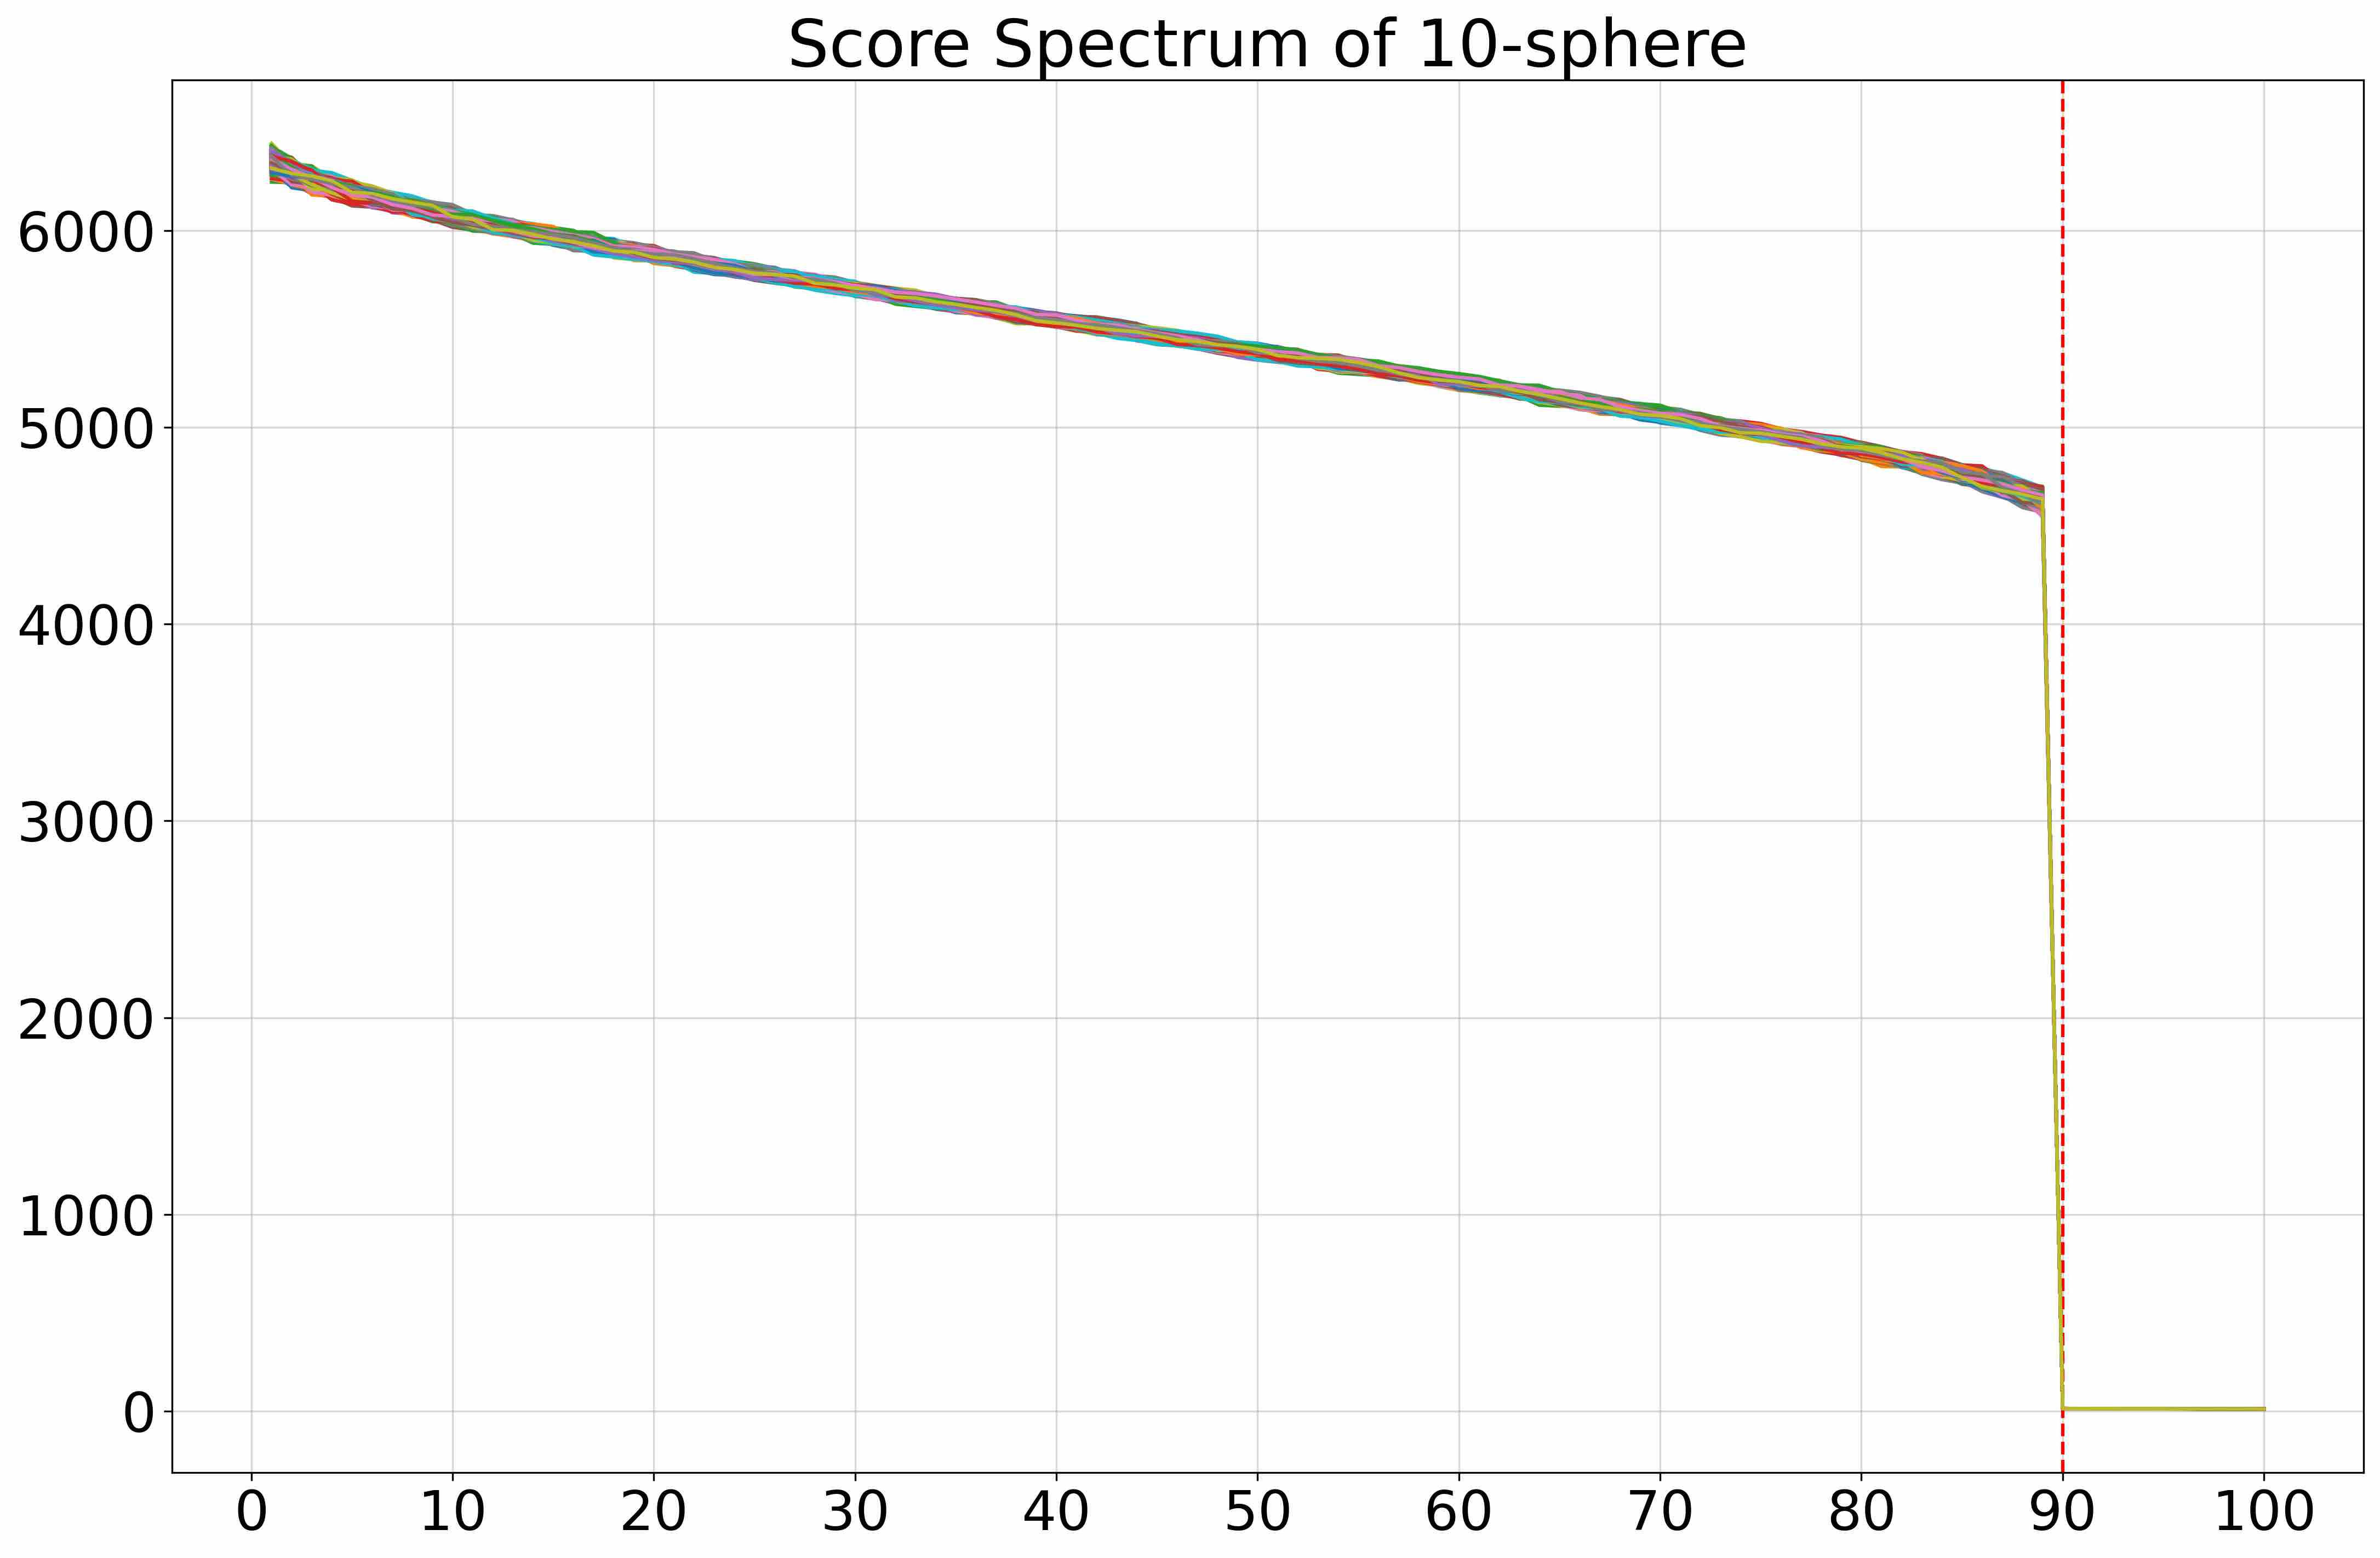
\includegraphics[width=\linewidth]{Chapter3/figures/10_sphere_spectrum.jpg}
        \caption{$k=10$}
        \label{ch3:fig:ksphere10}
    \end{subfigure}
    \hfill
    \begin{subfigure}[b]{0.49\linewidth}
        \centering
        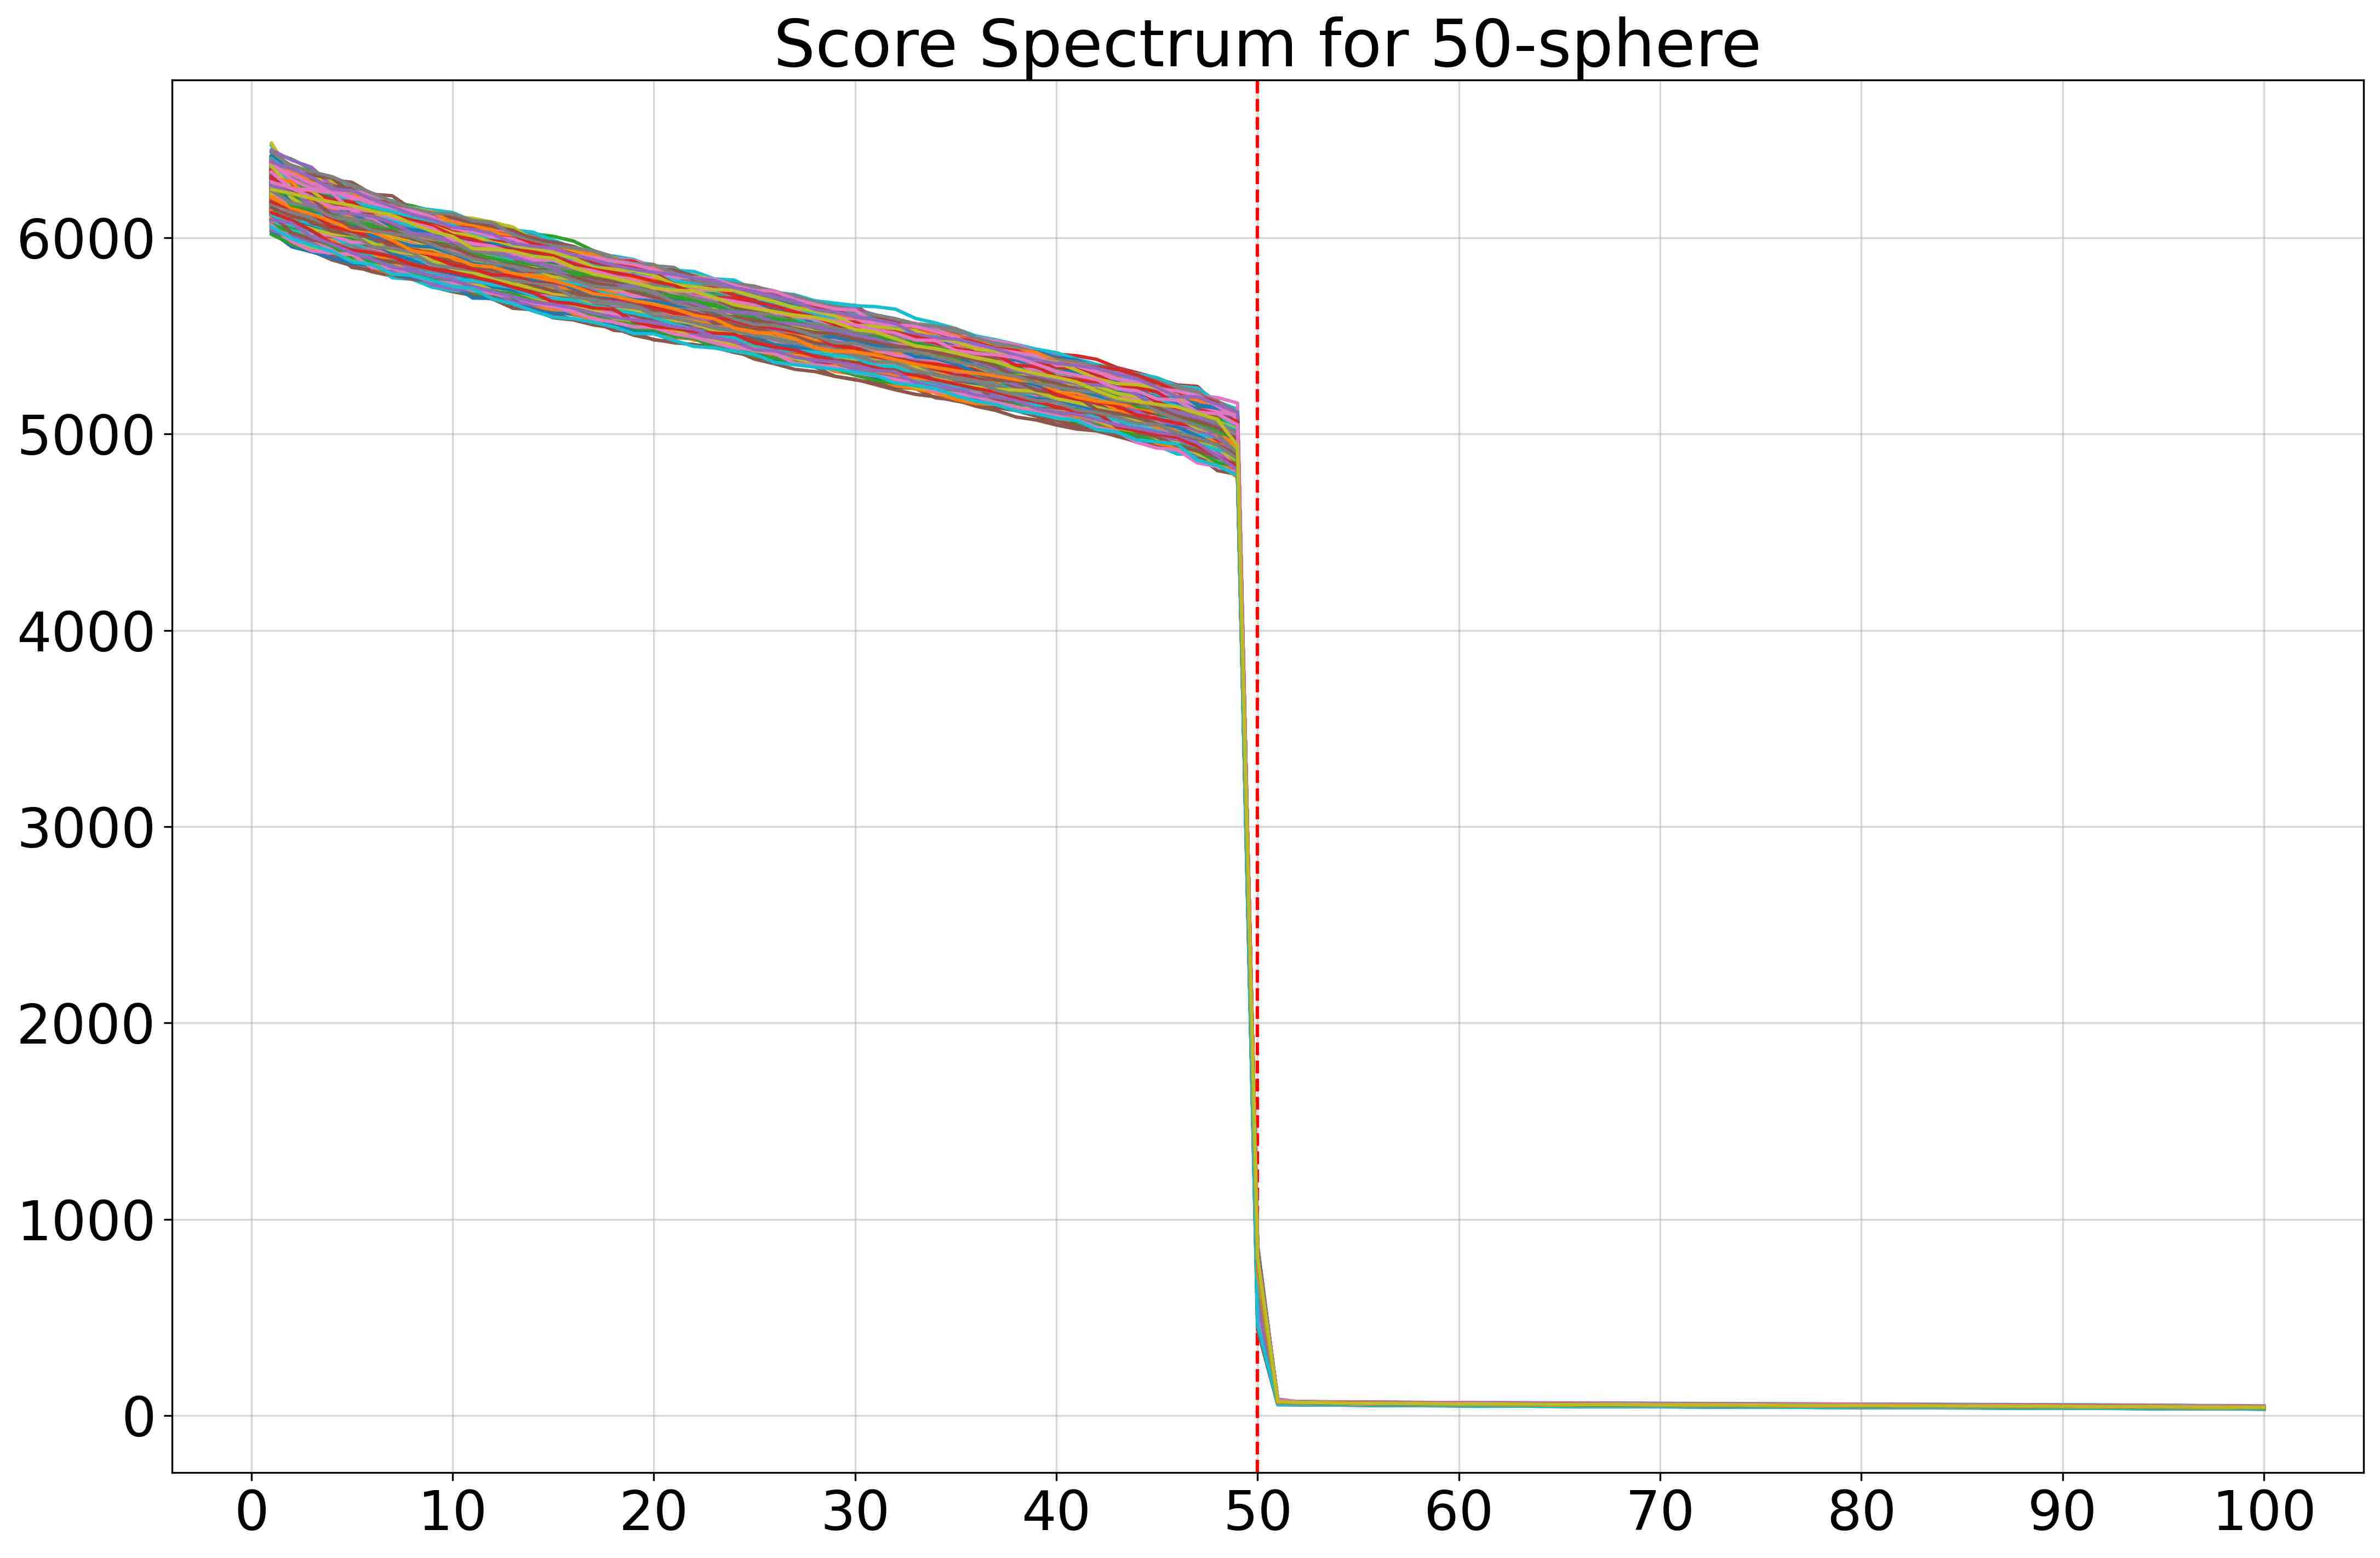
\includegraphics[width=\linewidth]{Chapter3/figures/50_sphere_spectrum.jpg}
        \caption{$k=50$}
        \label{ch3:fig:ksphere50}
    \end{subfigure}
    \caption{Singular values for the scores of $k$-sphere for $k=10, 50$. 
    In both cases around $k$ singular values almost vanish, clearly indicating the dimensionality of the manifold. Each line shows a score spectrum at different $\textbf{x}_0^{(j)}$.}
    \label{ch3:fig:ksphere}
\end{figure}

\textbf{Spaghetti line:} The intrinsic dimensionality of $k$-spheres could be well approximated by a linear dimensionality detection methods such as \cite{auto_ppca}. This is because these manifolds are contained in a low dimensional \textit{linear} subspace. In order to showcase the advantage of the \textit{non-linear} nature of our method we consider a \textit{spaghetti line} manifold. That is a curve $\tau \mapsto (\sin(\tau), \sin(2\tau), ..., \sin(100\tau))$ in a 100 dimensional ambient space, which is not contained in any low dimensional linear subspace (cf. Figure \ref{ch3:fig:line_samples} in Appendix \ref{ch3:appendix:additional_euclidean}). As expected, the linear method \cite{auto_ppca} greatly overstates the intrinsic dimension with a result of $\hat{k}_{\text{PPCA}}=98$. Yet, our approach utilizes the non-linear knowledge from the diffusion model to accurately predict an intrinsic dimensionality of one.  The score spectrum is presented in Figure \ref{ch3:fig:line} in Appendix \ref{ch3:appendix:additional_euclidean}.


\textbf{Union of $k$-spheres:} Due to the local nature of our method, we are able to generate an estimate $\hat{k}(\textbf{x}_0)$ of the intrinsic dimension around a given point $\textbf{x}_0$. This allows us to apply our approach to a union of manifolds and identify the dimension of each component. We illustrate this feature with the following experiment. We embed two spheres of different radii and dimensions in a 100 dimensional ambient space. First sphere has dimension $k_1 = 10$ and radius $r_1 = 1$ and the second sphere has $k_2=30$ and radius $r_2 = 0.25$\footnote{One can intuitively think of this manifold as a high-dimensional analog of a planet with a ring around it.}. We apply our method to this data using multiple $\textbf{x}_0^{(i)}$ randomly sampled from the dataset. We observe that our method produces a spectrum with two visible, separated drops. This indicates that the data comes from the union of manifolds of different dimensions. The resulting estimates are $\hat{k}_1 = 10$ and $\hat{k}_2=31$ depending on the chosen  $\textbf{x}_0^{(j)}$. The score spectra and the histogram of estimated dimensions are presented in Figures \ref{ch3:fig:unions_spectrum} and \ref{ch3:fig:union_dims} in Appendix \ref{ch3:appendix:additional_euclidean}.

\subsection{Experiments on image datasets}
\textbf{Synthetic image manifolds}: In this experiment, we investigated our method's ability to infer the dimension of synthetic image manifolds with known dimension. We crafted two synthetic image manifolds with controllable intrinsic dimension $k$: the "$k$ squares images manifold" and the "$k$ Gaussian blobs images manifold". The construction of these manifolds is detailed in Appendix \ref{ch3:Appendix:_design_of_synthetic_image_manifolds}. We evaluated our method on $k=$10, 20, and 100 dimensional manifolds for both types, with the score spectra and histograms of estimated dimensions for numerous data points displayed in Figures \ref{ch3:fig:squares_spectrum} and \ref{ch3:fig:gaussians_spectrum} in Appendix \ref{ch3:appendix:additional_image}.


On the squares image manifold, our method, ID-NF and PPCA consistently yielded accurate dimension estimates. PPCA's success on this dataset was anticipated since the manifold resides within a $k$-dimensional linear subspace.

On the more complex Gaussian blobs image manifold, our method stood out as the sole technique to consistently deliver accurate dimension estimates.  The accuracy of our method was not compromised by the manifold's increased complexity, unlike other methods. However, the estimation for the 100-dimensional manifold introduced some uncertainty, as indicated by a more leveled histogram and a less abrupt spectrum collapse (c.f. Figure \ref{ch3:fig:gaussians_spectrum}). This is attributed to the manifold's increased complexity and the inherent challenges in optimization, resulting in greater geometric and approximation errors.

\begin{figure}
    \begin{center}
        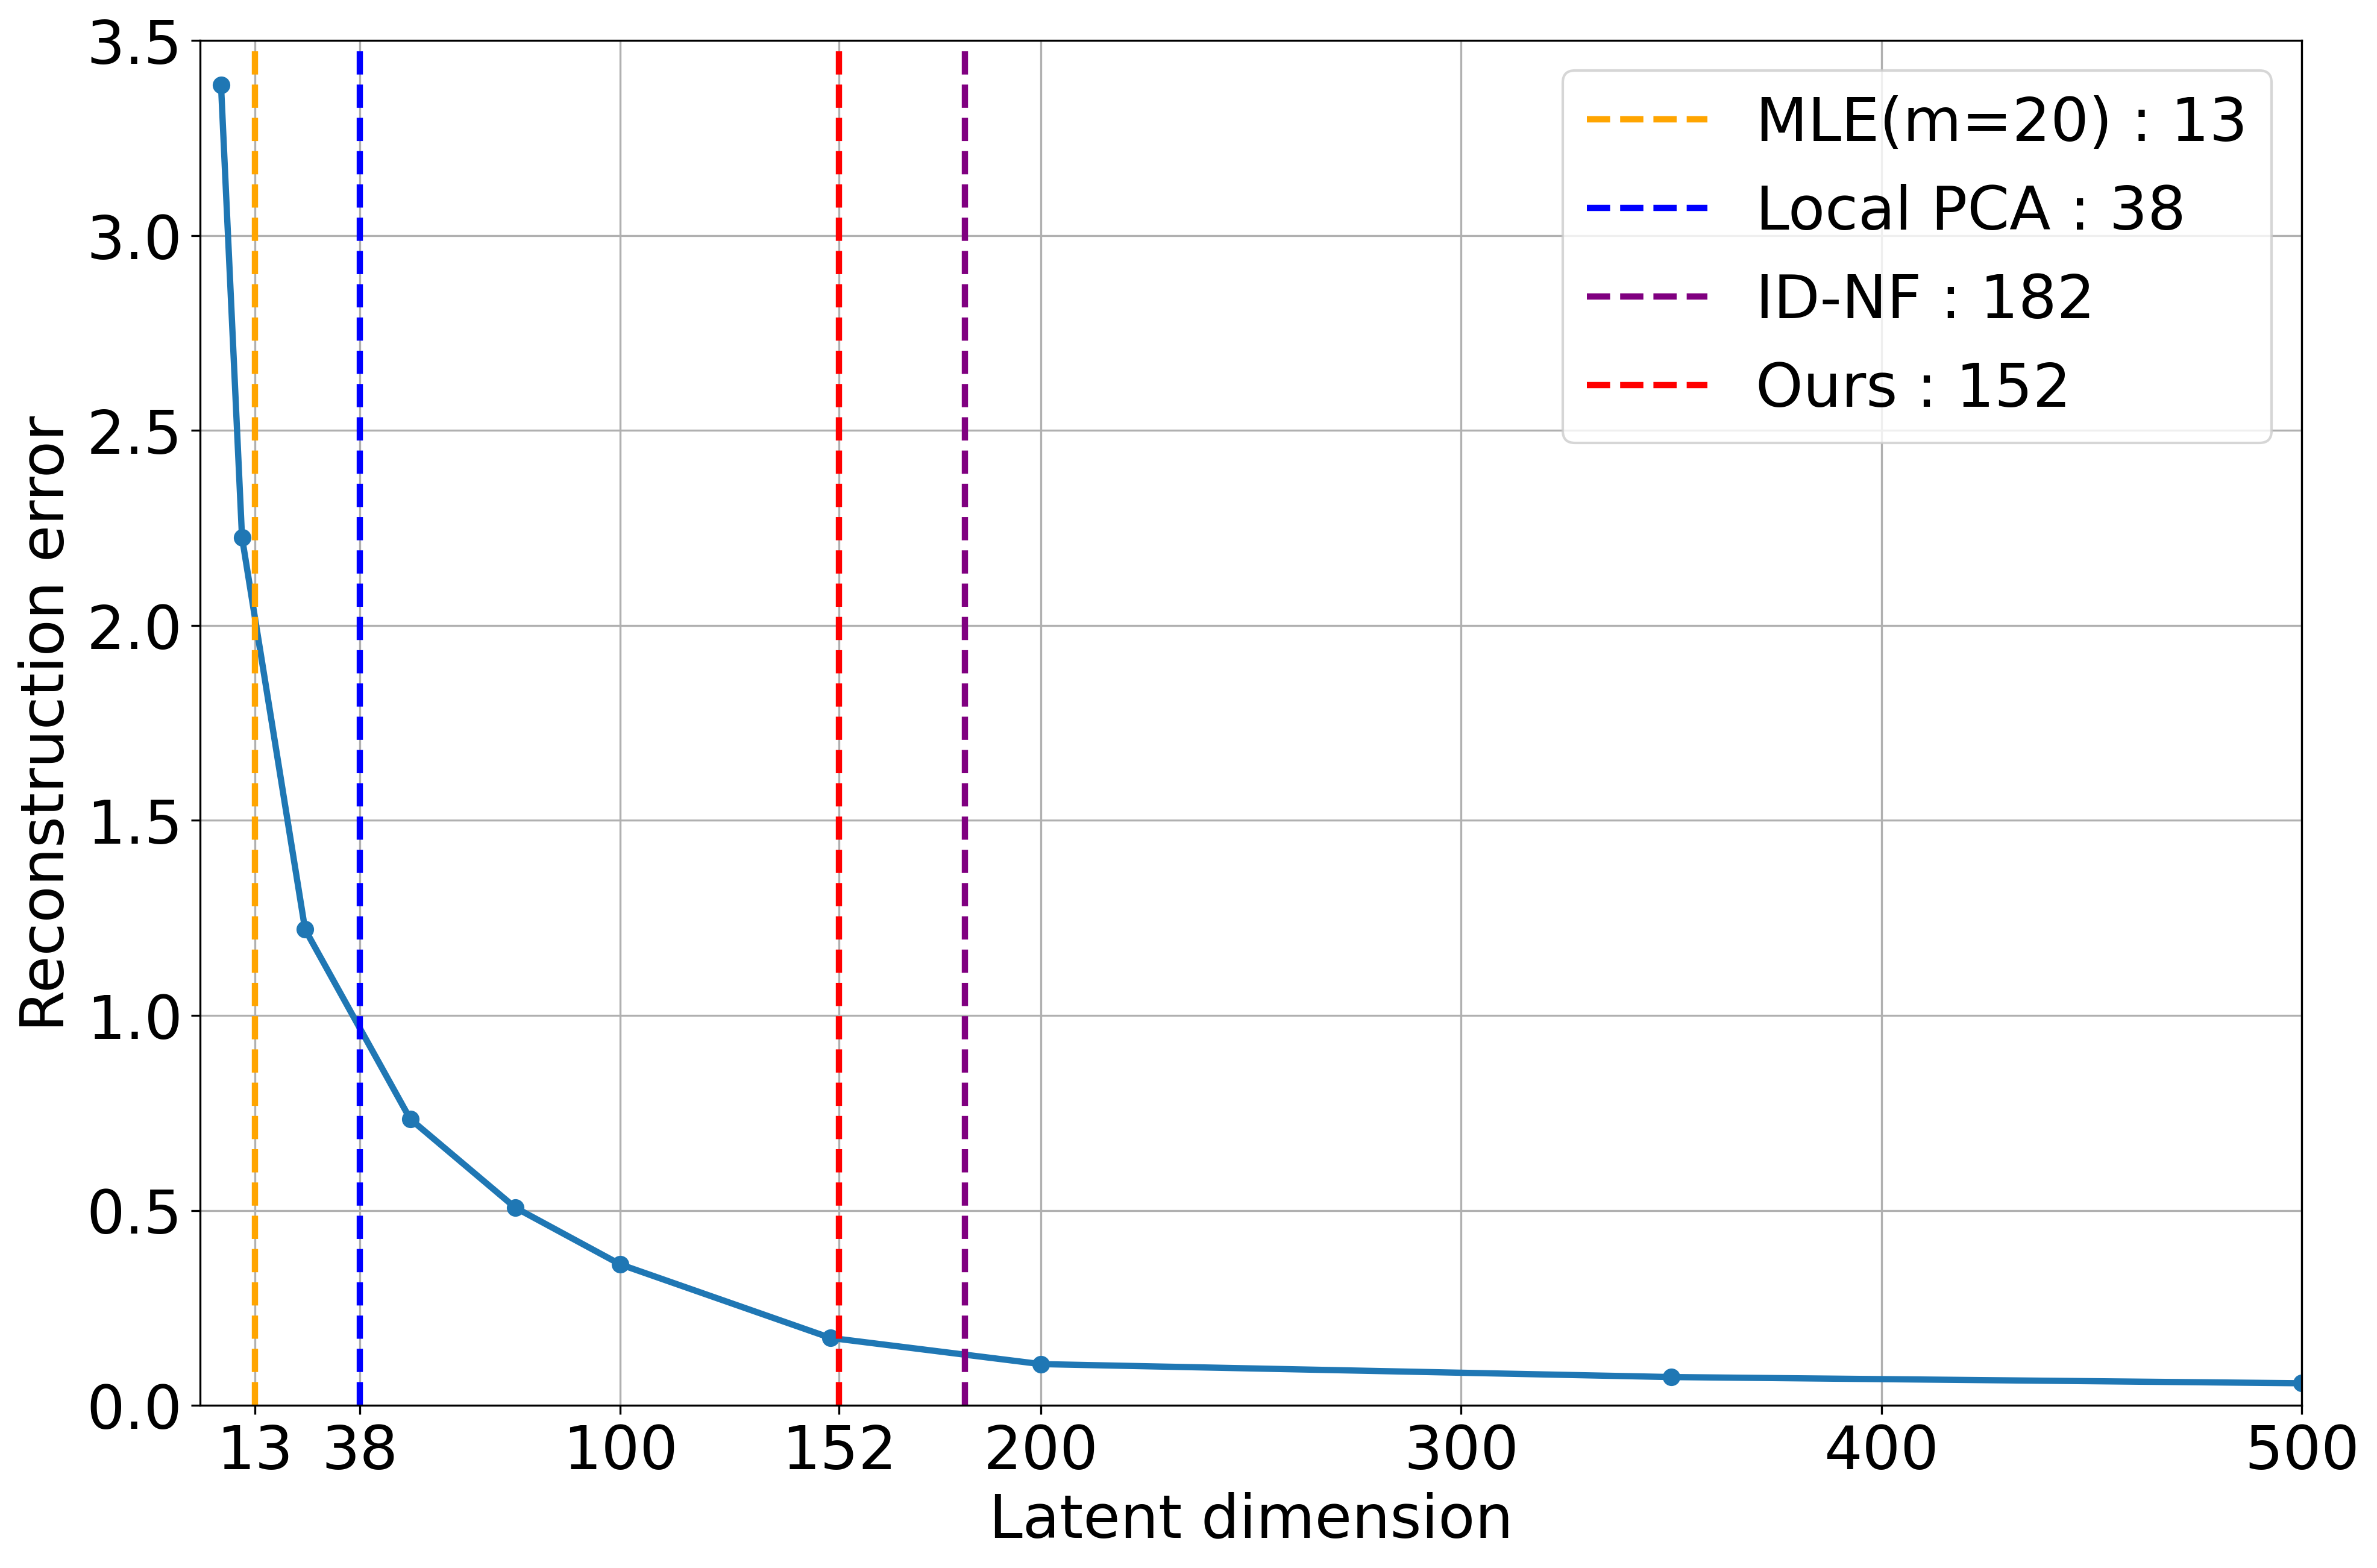
\includegraphics[width=0.75\textwidth]{Chapter3/figures/mnist_autoencoder.png}
        \caption{Auto-encoder reconstruction error on MNIST for different latent space dimensions. Vertical lines mark different estimations of intrinsic dimension.}
        \label{ch3:fig:mnist_autoencoder}
    \end{center}
\end{figure}


\textbf{MNIST:} In our study, we additionally applied the proposed technique to estimate the intrinsic dimension of the well-known MNIST dataset - an image dataset with an as-of-yet-undetermined intrinsic dimension. Our findings suggest that there exists a variation in the intrinsic dimensions across different digits. For instance, the digit `1' yielded an estimated dimension of 66, whereas the digit `9' exhibited a significantly higher estimated dimension of 152. This discrepancy can be attributed to the increased geometric complexity inherent to the digit `9'. Figure \ref{ch3:fig:score_spectra_mnist} elucidates these observations by displaying the score spectra which yielded the maximum estimated dimensions for each digit. We present the estimated dimension for each digit in Table \ref{ch3:tab:estimated_mnist_dimensions} and the complete set of spectra for each digit in the Appendix \ref{ch3:sec:Additional_Experimental_Results_for_MNIST}. 

We validate our estimates by comparing them with the reconstruction error of auto-encoders trained with different latent dimensions. As demonstrated in Figure 4, the ID estimate of our method is in close agreement with that of the ID-NF method, and both correlate with the point of diminishing returns on the reconstruction loss curve. This point marks a plateau in the effectiveness of additional latent dimensions to significantly reduce reconstruction error, further suggesting this point as the dataset's intrinsic dimension. In constrast, estimates produced by MLE and Local PCA are significantly lower, corresponding to regions of the curve where the reconstruction loss is still steeply decreasing. This suggests these methods underestimate the manifold dimension. These findings call for a careful interpretation of the intrinsic dimension estimates of popular machine learning datasets provided by \cite{pope2021intrinsic}, as they rely on the MLE method, which we have found to consistently underestimate manifold dimensions. On the other hand, PPCA notably overestimated the dimension, with $\hat{k}_{\text{PPCA}} = 706$.



\begin{figure*}
    \centering
    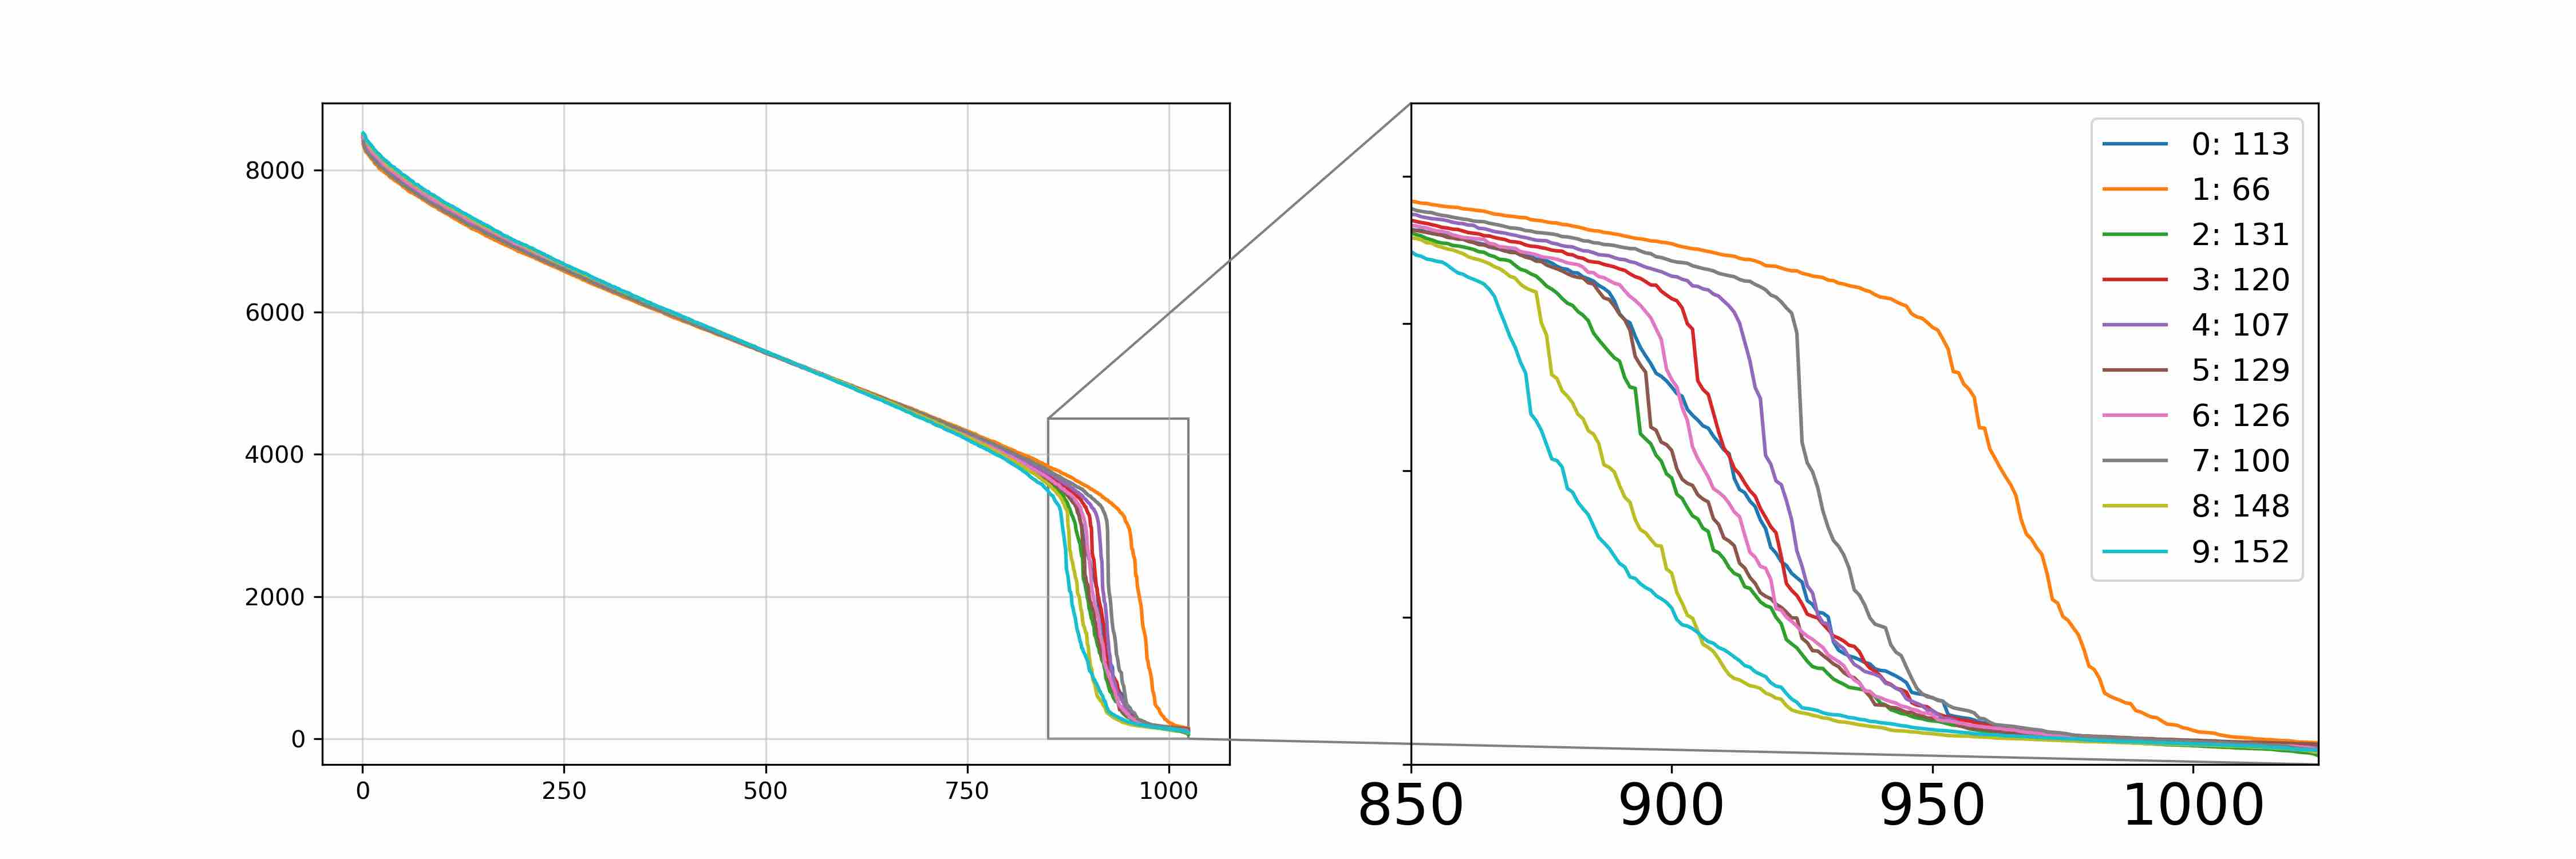
\includegraphics[width=0.99\textwidth]{Chapter3/figures/image_manifolds/MNIST/mnist_spectrum.jpg}
    \caption{MNIST score spectra that yielded the highest estimated dimension for each digit}
    \label{ch3:fig:score_spectra_mnist}
\end{figure*}

    
\begin{table}[ht]
    \centering
    \footnotesize
    \setlength{\tabcolsep}{4pt} 
    \renewcommand{\arraystretch}{0.9} 
    \begin{tabular}{c|c|c|c|c|c|c|c|c|c}
    \toprule
    0 & 1 & 2 & 3 & 4 & 5 & 6 & 7 & 8 & 9 \\
    \midrule
    113 & 66 & 131 & 120 & 107 & 129 & 126 & 100 & 148 & 152 \\
    \bottomrule
    \end{tabular}
    \vspace{8pt} % This adds space between the table and the caption
    \caption{Estimated intrinsic dimension for each MNIST digit}
    \label{ch3:tab:estimated_mnist_dimensions}
    \end{table}
    
    \begin{table}[ht]
    \centering
    \resizebox{\columnwidth}{!}{ 
    \begin{tabular}{lccccccc}
    \toprule
    & Ground Truth & Ours & ID-NF & MLE (m=5) & MLE (m=20) & Local PCA & PPCA \\
    \midrule
    Euclidean Data Manifolds & & & & & & & \\
    \quad 10-sphere &10 &11 &11 &9.61 &9.46 &11 &11 \\
    \quad 50-sphere &50 &51 &51 &35.52 &34.04 &51 &51 \\
    \quad Spaghetti line &1 &1 &1 &1.01 &1.00 &32 &98 \\
    \midrule
    Image Manifolds & & & & & & & \\
    \quad Squares & & & & & & & \\
    \qquad $k=10$ &10 &11 &9.7 &8.48 &8.17 &10 &10 \\
    \qquad $k=20$ &20 &22 &19.5 &14.96 &14.36 &20 &20 \\
    \qquad $k=100$ &100 &100 &94.2 &37.69 &34.42 &78 &99 \\
    \quad Gaussian blobs & & & & & & & \\
    \qquad $k=10$ &10 &12 &9.8 &8.88 &8.67 &10 &136 \\
    \qquad $k=20$ &20 &21 &17.8 &16.34 &15.75 &20 &264 \\
    \qquad $k=100$ &100 &98 & 56.3 &39.66 &35.31 &18 &985 \\
    \midrule
    MNIST &N/A &152 &182 &14.12 &13.27 &38 &706 \\
    \bottomrule
    \end{tabular}
    }
    \vspace{8pt} % This adds space between the table and the caption
    \caption{Comparison of dimensionality detection methods on various data manifolds.}
    \label{ch3:tbl:results}
    \end{table}
    

\section{Conclusions and further directions}
\label{ch3:sec:conclusions}
In this work, we proved theoretically and confirmed experimentally that diffusion models can infer the intrinsic dimension from the data. We introduced an approach that estimates the intrinsic dimension of the data manifold from a pre-trained diffusion model. This approach capitalizes on the observation that, the diffusion model evaluated at sufficiently small diffusion time approximates the normal bundle of the data manifold.  Our work offers a twofold contribution: it highlights that diffusion model detects the lower dimensional structure of data and provides a rigorous method for intrinsic dimension estimation. 

We conducted a rigorous comparison of three types of ID estimators: traditional statistical methods, normalizing flow-based techniques, and our diffusion-based approach. Our findings consistently show that for high-ID datasets, methods leveraging neural networks' inductive biases are superior. Notably, our diffusion-based method emerges as the most effective, owing to its enhanced training stability and freedom from the architectural constraints of normalizing flows.

Furthermore, our research introduces new estimates for the MNIST's dimensionality, demonstrating strong alignment with the predictions of an auto-encoder trained across a range of latent dimensions.% Our results challenge the traditionally accepted MNIST dimensionality estimates \cite{pope2021intrinsic}, revealing them as considerable underestimations and prompting a reevaluation of our understanding of such datasets.

%We are the first, to our knowledge, to present an intrinsic dimension estimation method based on diffusion models. The superior performance of our approach on higher dimensional manifolds compared to statistical estimators is attributed to the enhanced statistical efficiency from the inductive biases in the neural network architectures approximating the score function.  
Our work opens new paths for understanding and estimating intrinsic data dimension, with potential implications across the field of machine learning. Future research should explore this method's applicability to other data types and its potential across various domains.

\section*{Impact Statement}
This paper presents work whose goal is to advance the field of Machine Learning. There are many potential societal consequences of our work, none which we feel must be specifically highlighted here.

\section*{Acknowledgements}
JS aknowledges support from the Cantab Capital Institute for the Mathematics of Information and Aviva. GB acknowledges support from GSK. TD acknowledges support from the EPSRC programme grant in `The Mathematics of Deep Learning', under the project EP/L015684/1. CBS acknowledges support from the Philip Leverhulme Prize, the Royal Society Wolfson Fellowship, the EPSRC advanced career fellowship EP/V029428/1, the EPSRC programme grant EP/V026259/1, and the EPSRC grants EP/S026045/1 and EP/T003553/1, EP/N014588/1, EP/T017961/1, the Wellcome Innovator Awards 215733/Z/19/Z and 221633/Z/20/Z, the European Union Horizon 2020 research and innovation programme under the Marie Skodowska-Curie grant agreement No. 777826 NoMADS, the Cantab Capital Institute for the Mathematics of Information and the Alan Turing Institute. This research was supported by the NIHR Cambridge Biomedical Research Centre (NIHR203312). The views expressed are those of the author(s) and not necessarily those of the NIHR or the Department of Health and Social Care.
